%% {\centering
%% 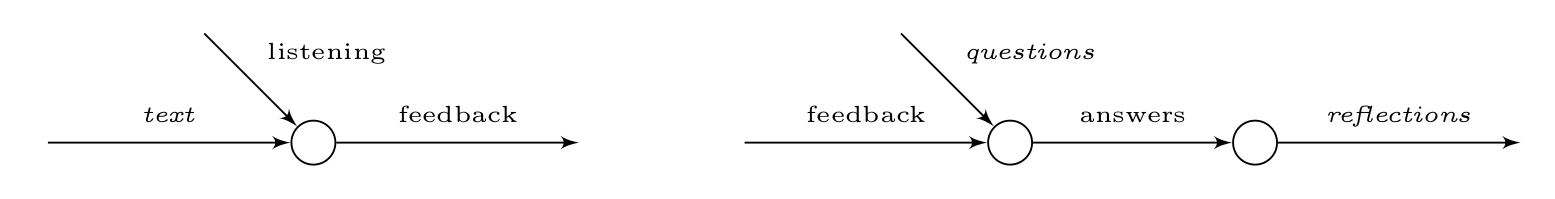
\includegraphics[width=.9\textwidth]{ww-serendipity-diagram}
%% \par}

Italicised elements (\emph{presentation}, \emph{questions}, and
\emph{reflections}) are the responsibilities of the presenting author; the other
elements (listening, feedback, and answers) are the responsibilities of the attendant critics.
%
\begin{figure}
{\centering
\begin{tikzpicture}[
single/.style={draw, anchor=text, rectangle},
]
\node (discovery) {\textbf{\emph{Discovery:}}};
% poet generates poem
\node[single, right=8mm of discovery.east,text width=1.5cm] (poet) {\emph{poetry generator}};
\node[single, right=4mm of poet.east] (poem) {P};
\draw [-latex] (poet.east) -- (poem.west);
% critic listens to poem and offers feedback
\node[single, right=4mm of poem.east,text width=1.5cm] (critic) {comment generator};
\draw [-latex] (poem.east) -- (critic.west);
\node[single, right=4mm of critic.east] (feedback) {F};
\draw [-latex] (critic.east) -- (feedback.west);

%%% Next phase
\node[below=1cm of discovery] (invention) {\textbf{\emph{Invention:}}};
% poet integrates feedback
\node[single, right=8mm of invention.east] (feedbackcont) {F};
\node[single, right=8mm of feedbackcont.east,text width=1.7cm] (integrator) {\emph{feedback integrator}};
\draw [-latex] (feedbackcont.east) -- (integrator.west);

\node[single, below=8mm of integrator.south,text width=1.5cm] (explainer) {feedback explainer};

\node[single, below right=2mm and 2mm of integrator] (question) {Q};
\node[single, below left=2mm and 2mm of integrator] (answer) {A};

\draw[-latex] ([yshift=-1.5mm]integrator.east) to [out=0,in=90] (question.north) ;
\draw[-latex] (question.south) to [out=270,in=0] (explainer.east) ;
\draw[-latex] (explainer.west) to [out=180,in=270] (answer.south) ;
\draw[-latex] (answer.north) to [out=90,in=180] ([yshift=-1.5mm]integrator.west) ;

\node[single, right=8mm of integrator.east] (problem) {X};

\draw [-latex] (integrator.east) -- (problem.west);

% poet reflects on feedback and updates codebase

\node[single, right=4mm of problem.east,text width=1.5cm] (pgrammer) {\emph{code}\\ \emph{generator}};

\draw [-latex] (problem.east) -- (pgrammer.west);

\node[single, right=4mm of pgrammer.east,text width=.3cm] (etc) {...};

\draw [-latex] (pgrammer.east) -- (etc.west);
\end{tikzpicture}


\par}
\caption{Generative schematic for a Writers Workshop\label{fig:generative-diagram}}
\end{figure}
%
The system as a whole can be further decomposed into generative
components, as in Figure \ref{fig:generative-diagram}.
